\subsection{Greedy Heuristic Path}\label{sec:greedy}
As mentioned in (ref LP) finding a optimal solution of a path is a NP-complete problem. NP-complete problems are as of today very expensive to solve optimally. In this section a greedy approach is taken, which solves the problem one edge at a time instead of trying to give a global solution to an entire path.  

Given a path $P = \langle u_1,u_2,\dots,u_k \rangle$. In measuring the fastest way to pass an edge on the path, there are two probable cases:
\begin{enumerate}
	\item It is fastest to drive
	\item It is fastest to charge, and then drive
\end{enumerate}

The intuition is then to figure out the time we will spend for both of these cases and picking the fastest option. However, it might not be possible to only drive, given the limited battery of the EV. The optimal speed when passing the edge $(u_i, u_j)$ without charging, can be found by solving this equation for $v$:
\[B_{cur} - D(u_i, u_j) * R_{CO}(v) = 0\] 
We call this speed $v_{opt}$. If $v_{opt}$ is lower than $v_{min}(e)$, the minimum speed of the edge, there is not enough energy in the battery to drive from $u_i$ to $u_j$ and thus the time is set to $-\infty$ indicating that just driving is not an option. If it is possible to drive the edge using the only energy from the battery the time it will take to pass the edge can be calculated as:
 \[T = \frac{D((u_i, u_j))}{v_{opt}} \] 
The time spent passing an edge $(u_i, u_j)$ while charging first, is given by the following equation:

\begin{equation*}
\begin{aligned}
 & T(v,(u_i, u_j)) = \frac{D((u_i, u_j))}{v} + \frac{R_{CO}(v) * D((u_i, u_j)) - B_{cur}}{charge_{rate}(u_j)}
\end{aligned}
\end{equation*}\label{eq:drivingAndCharging}

Where $v$ is the speed of the vehicle, $D(u_i, u_j)$ is the distance between vertices $u_i$ and $u_j$, $R_{CO}(v)$ is the consumption rate of the EV, $B_{cur}$ is the current battery of the vehicle. Since we only charge exactly enough to pass an edge, there might be charging stations previous to $u_i$ which we could have charged more at without exceeding the battery capacity. Thus we would go back in history and charge at the best previous charge stations, recursively, until we have enough energy to pass $(u_i, u_j)$ this is done by $charge_{rate}(u_j)$ which gives the charge rate of the best charge previous to $u_j$.

The above equation yields a function of the form: $av^2 + bv + c$, due to the fact that $R_{CO}(v)$ is a quadratic function. $a$, $b$ and $c$ are some constants which are given by the instance of the vehicle. Represented in a Cartesian coordinate system, $T(v,(u_i, u_j)))$ is a parabola, as can be seen in Figure \ref{graph}, note that the graph is only defined for positive speeds larger than $0$ and can only be calculated if $charge_{rate}(u_j)$ is larger than $0$. On the x-axis is the speed of the vehicle and on the y-axis is the time spent. The turning point of the graph represents the optimal speed to drive for the given edge, denoted as $v_{opt}(e)$. The point is easily calculated by finding a tangent line with a slope of $0$. If $v_{opt}(e)$ is smaller than $v_{min}(e)$, then $v_{min}(e)$ defines the optimal speed for the edge. Similarly if $v_{opt}(e)$ is larger than $v_{max}(e)$, $v_{max}(e)$ defines the optimal speed for the edge. If $v_{opt}(e) == v_{min}(e)$ there might be a possibility that driving and charging is not an option. 

\begin{figure}[!htb]
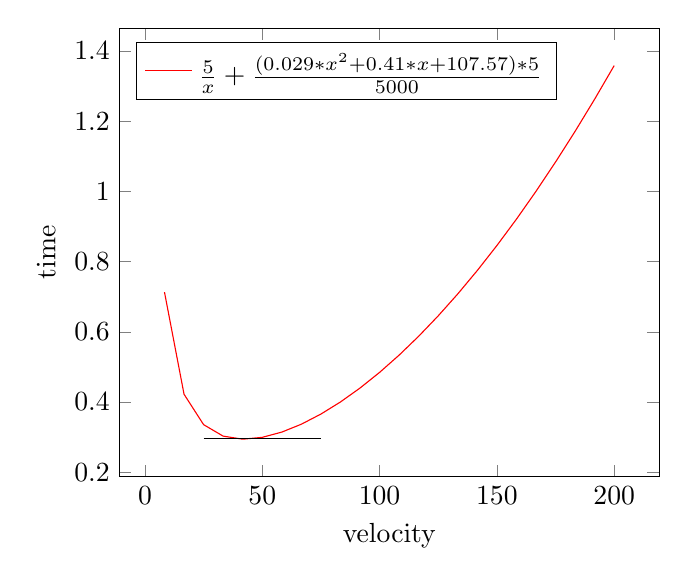
\begin{tikzpicture}
\begin{axis}[xlabel=velocity, ylabel=time,legend style={legend pos=north west}]
\addplot[draw=red,domain=0:200]{(5/x)+(((0.0286*x^2 + 0.4096*x + 107.57)*5)/5000)};
\addlegendentry{$\frac{5}{x}+\frac{(0.029*x^2 + 0.41*x + 107.57)*5}{5000}$}

\addplot[draw=black,domain=25:75]{0.295};
% \addplot[mark=*, domain=25:75] coordinates {(37,295)};
\end{axis}
\end{tikzpicture}% 
\caption{In this instance of $T(v,(u_1, u_2))$, going from $u_1$ to $u_2$, we have a distance of $5 \si{\km}$ and a charge speed of $5 \si{\kW}$ on $u_1$. The optimal speed in this case is $42.12\si{\km\per\hour}$, and the total time is roughly 17 minutes to pass through the edge when driving and charging}
\end{figure}\label{graph}
Having the two ways of deciding the time it takes to pass an edge a algorithm can be created which decide how to drive each road segment can be formulated.   

\begin{algorithmic}[1]
\Function{travel\_time}{$RN, u_1, u_2, EV$}
	\State $e = (u_1, u_2)$
	\State $v_{opt1} = solve1\langle v, e, EV.B_{cur}-RN.D(e)*EV.R_{CO}(v)\rangle$
	\If{$ u_1.B_{cur} - RN.D(e)*EV.R_{CO}(v_{opt1}) < 0 $}
		\State $time_1 = \infty$
	\Else
		\State $time_1 = RN.D(e) / v_{opt1}$
		\State $energy\_used_{1} = RN.D(e)*EV.R_{CO}(v_{opt1})$
	\EndIf
		\State $CS = getCS(u_1, u_2)$ 
		\State $energy\_needed_{2} = \infty$
		\State $energy = u_1.B_{cur}$
		\State $time\_added = 0$
		\State $time_2 = \infty$
	\While{$energy\_needed_{2} > energy  \And  len(CS) \neq 0$}
		\State $best_{CS} = extractmax(CS)$
		\State $B_{possible} = best_{CS}.B_{possible}$
		\State $charge\_rate = RN.R_{CH}(best_{CS})$
		\State $v_{opt2} = solve2 \langle v, e,  RN.D(e)/v + (RN.D(e)* 
			EV.R_{CO}(v)-energy)/charge\_rate) \rangle$
		\State $energy\_needed_{2} = RN.D(e)*EV.R_{CO}(v_{opt2})$
		\State $energy = energy + B_{possible}$
		\If{$energy - energy\_needed_{2}) < 0$}
			\State $time\_added = time\_added + B_{possible}/charge\_rate$
			\State $CS.remove(0)$
			\State $updateCS(CS)$
		\EndIf	
	\EndWhile
	\If{$energy - energy\_needed_{2}) < 0$}
		\State $time_2 = (RN.D(e)/*v_{opt2}) + (energy\_needed_{2}/charge\_rate) + time\_added$
	\EndIf
	%\if{$time_1 == \infty \And time_2 == \infty$}
	%	\State \Return $\infty, NIL, \infty$
	%\Endif
	\If{$time_1 <= time_2$}
		\State \Return $time_1, CS, energy\_used_1$
	\Else
		\State \Return $time_2, CS, energy\_used_2$
	\EndIf

\EndFunction
\end{algorithmic}\label{alg:fastest_path}

The $travel\_time$ function takes as input a road network $RN$, the two vertices which makes up the edge to be driven and the EV which drives the path. The function uses a few helping functions, the two solve functions $solve1$ and $solve2$ are solvers specified for each of the cases and returns the optimal speed of the EV within the speed limit of the edges driven. The function $getCS(u_1, u_2)$ returns a list of charge stations. If $u_1$ is a charge stations with a higher charge rate than any charge station previous to $u_1$ then $u_1$ is returned otherwise $u_1$ is append to the list of charging stations previous to $u_1$, this ensure that the charge station with the best charge rate is alway the 1st in the list of previous charge stations. The last function $updateCS(CS)$ finds a new best charge station and deletes all charge stations prior to it, this is need because the best charge station have been removed by $CS.remove(0)$. Lines 3-8 handles case 1: Driving using the battery already in the battery. Lines 9-26 handles case 2: Driving and charging. The while loop ranging from line 14 till 24 makes sure the EV always charge as much as possible at the best previous charge station, with out allowing over charging of the battery. The if statement on line 4 and 25 check is a valid solution to the case is found, if so it the time for the case is calculated. Lines 27-32 if a solution is found and it so which solution is better. Having a way to solve a single edge the time of the path can be decided by looping through all edges form $e_1$ to $e_n$
